%%%%%%%%%%%%%%%%%%%%%%% file template.tex %%%%%%%%%%%%%%%%%%%%%%%%%
%
% This is a general template file for the LaTeX package SVJour3
% for Springer journals.          Springer Heidelberg 2010/09/16
%
% Copy it to a new file with a new name and use it as the basis
% for your article. Delete % signs as needed.
%
% This template includes a few options for different layouts and
% content for various journals. Please consult a previous issue of
% your journal as needed.
%
%%%%%%%%%%%%%%%%%%%%%%%%%%%%%%%%%%%%%%%%%%%%%%%%%%%%%%%%%%%%%%%%%%%
%
%
\RequirePackage{fix-cm}
%
%\documentclass{svjour3}                     % onecolumn (standard format)
%\documentclass[smallcondensed]{svjour3}     % onecolumn (ditto)
%\documentclass[smallextended]{svjour3}       % onecolumn (second format)
\documentclass[twocolumn]{svjour3}          % twocolumn
%
\smartqed  % flush right qed marks, e.g. at end of proof
%
\usepackage{graphicx}
\usepackage[hidelinks]{hyperref}
\usepackage[utf8]{inputenc}
\usepackage[T1]{fontenc}
\usepackage{csquotes}
%
% \usepackage{mathptmx}      % use Times fonts if available on your TeX system
%
% insert here the call for the packages your document requires
%\usepackage{latexsym}
% etc.
%
% please place your own definitions here and don't use \def but
% \newcommand{}{}
%
% Insert the name of "your journal" with
% \journalname{myjournal}
%

% TODOS: =========================================
% KILIAN: affmark, affaddr, wasn't defined and I'm not sure about it's purpose, so I'm
% filling this in for now: 
% (copied from https://tex.stackexchange.com/questions/9594/)
\newcommand*{\affaddr}[1]{#1} % No op here. Customize it for different styles.
\newcommand*{\affmark}[1][*]{\textsuperscript{#1}}
% KILIAN: \Letter wasn't defined, so I'm telling LaTeX to ignore it
\newcommand*{\Letter}{\relax}
% ==================================================
\begin{document}

\title{Software Training in HEP%\thanks{Grants or other notes
%about the article that should go on the front page should be
%placed here. General acknowledgments should be placed at the end of the article.}
}
%\subtitle{Do you have a subtitle?\\ If so, write it here}

%\titlerunning{Short form of title}        % if too long for running head

\author{Sudhir Malik  (editor)~\protect\affmark[1] % ORCID: 0000-0002-6356-2655
\and
Samuel Meehan \affmark[2]
\and
Kilian Lieret\affmark[3] % ORCID: 0000-0003-2792-7511
\and
Meirin Oan~Evans\affmark[4]
\and
Michel H.\ Villanueva\affmark[5]
\and
Daniel S.\ Katz\affmark[6] % ORCID: 0000-0001-5934-7525
\and
Graeme A.\ Stewart\affmark[2] % ORCID: 0000-0003-0182-7088
\and
Peter Elmer\affmark[7]
% --- sort alphabetically from here
\and
David Chamont\affmark[8] % ORCID: 0000-0003-2618-7355
\and
Stefan Roiser\affmark[2] % ORCID: 0000-0002-5600-8592
\and
Andrea Valassi\affmark[2] % ORCID: 0000-0001-9322-9565
\and
Clemens Lange\affmark[2] % ORCID: 0000-0002-3632-3157
\and
Amber Roepe\affmark[34] % ORCID: 0000-0001-5933-9357
\and
Giordon Stark\affmark[9] % 0000-0001-6616-3433
\and
Judita ~Mamu{\v{z}}i{\'{c}}\affmark[10] % 0000-0002-3203-4243
\and
Arturo S\'{a}nchez Pineda\affmark[11] % 0000-0001-8241-7835
\and
Philipp Gadow\affmark[12] % ORCID: 0000-0003-4475-6734
\and
Robin Newhouse\affmark[13]
\and
Scarlet Norberg\affmark[1]
\and
Emery Nibigira\affmark[14]
\and
Savannah Thais\affmark[7]
\and
Matthew Feickert\affmark[6]% ORCID: 0000-0003-4124-7862
\and
Daniel Guest\affmark[15]
\and
Maximilian M. Horzela\affmark[16]% ORCID: 0000-0002-3190-7962
\and
Konstantin Lehmann\affmark[17] % ORCID: 0000-0002-8590-8231
\and
Stefan Wunsch\affmark[2,16]
\and
Lukas Heinrich\affmark[2]
\and
Henry Schreiner\affmark[7]
\and
Matthew Bellis\affmark[18] % ORCID: 0000-0002-6353-6043
\and
Mason Proffitt\affmark[19] % https://orcid.org/0000-0003-0323-8252
\and
Stephen Nicholas Swatman\affmark[2,20]
\and
Oksana Shadura\affmark[21] %ORCID: 0000-0001-5356-2494
\and
Kevin Nelson\affmark[22] %ORCID: 0000-0003-4194-1790
\and
Brendan Regnery\affmark[23]
\and
Johan Sebastian Bonilla\affmark[23]
\and
Angela Burger\affmark[24] %ORCID: 0000-0003-0685-4122
\and
Ke Li\affmark[19]
\and
Riccardo Maria Bianchi\affmark[25] %ORCID: 0000-0001-7345-7798 
\and
Marc Huwiler\affmark[26]
\and
Jackson Burzynski\affmark[27]
\and
Devdatta Majumder\affmark[28]
\and
Siqi Yuan\affmark[29]
\and
Gianluca Bianco\affmark[30,31]
\and
David Yakobovitch\affmark[32]
\and
Sizar Aziz\affmark[8]
\and
Stephan Hageboeck\affmark[2] %ORCID: 0000-0001-9359-2196
\and
Bernhard Manfred Gruber\affmark[2,35,36] %ORCID: 0000-0001-7848-1690
}

\authorrunning{The HSF Training WG}

\institute{
\Letter Sudhir Malik\\
sudhir.malik@upr.edu\\
\\
\affaddr{\affmark[1]University of Puerto Rico Mayaguez, USA}\\
\affaddr{\affmark[2]CERN, Geneva, Switzerland}\\
\affaddr{\affmark[3]Ludwig Maximilian University of Munich, Germany}\\
\affaddr{\affmark[4]University of Sussex, Brighton, UK}\\
\affaddr{\affmark[5]University of Mississippi, Oxford, MS, USA}\\
\affaddr{\affmark[6]University of Illinois at Urbana-Champaign, IL, USA}\\
\affaddr{\affmark[7]Princeton University, Princeton, NJ, USA}\\
\affaddr{\affmark[8]Universit\' e Paris-Saclay, CNRS/IN2P3, IJCLab, Orsay, France}\\
\affaddr{\affmark[9]Santa Cruz Institute for Particle Physics, UC Santa Cruz, CA, USA}\\
\affaddr{\affmark[10]Instituto de F\' ssica Corpuscular / Consejo Superior de Investigaciones Cient\' ificas - University of Valencia (IFIC / CSIC - UV), Spain }\\
\affaddr{\affmark[11]LAPP, Universit\'e Savoie Mont Blanc, CNRS/IN2P3, Annecy, France
}\\
\affaddr{\affmark[12]Deutsches Elektronen-Synchrotron DESY, Hamburg, Germany }\\
\affaddr{\affmark[13]University of British Columbia, Vancouver, Canada }\\
\affaddr{\affmark[14]Universit\'e de Strasbourg, CNRS, IPHC UMR 7178, Strasbourg, France }\\
\affaddr{\affmark[15]Humboldt University of Berlin, Berlin, Germany }\\
\affaddr{\affmark[16]Karlsruhe Institute of Technology (KIT), Karlsruhe, Germany }\\
\affaddr{\affmark[17]Simon Fraser University, Burnaby BC, Canada }\\
\affaddr{\affmark[18]Siena College, Loudonville, NY, USA }\\
\affaddr{\affmark[19]University of Washington, Seattle, WA, USA }\\
\affaddr{\affmark[20]University of Amsterdam, Amsterdam, The Netherlands }\\
\affaddr{\affmark[21]University of Nebraska, Lincoln, NE, USA }\\
\affaddr{\affmark[22]University of Michigan, Ann Arbor, MI, USA }\\
\affaddr{\affmark[23]University of California Davis, Davis, CA, USA }\\
\affaddr{\affmark[24]Oklahoma State University, Stillwater, OK 74078, USA }\\
\affaddr{\affmark[25]University of Pittsburgh, Pittsburgh, PA, USA }\\
\affaddr{\affmark[26]Universität Zürich, Zürich, Switzerland }\\
\affaddr{\affmark[27]University of Massachusetts, Amherst MA, USA }\\
\affaddr{\affmark[28]Institut Ruđer Bo\v skovi\' c, Zagreb, Croatia }\\
\affaddr{\affmark[29]Boston University, Boston, USA }\\
\affaddr{\affmark[30]University of Bologna, Bologna, Italy }\\
\affaddr{\affmark[31]INFN (Istituto Nazionale di Fisica Nucleare), Italy }\\
\affaddr{\affmark[32]SingleStore, New York}\\
\affaddr{\affmark[34]University of Oklahoma, Norman, OK, USA } \\
\affaddr{\affmark[35]Center for Advanced Systems Understanding, Saxony, Germany}\\
\affaddr{\affmark[36]Technische Universität Dresden, Dresden, Germany }\\
}





%%%%%%%%%%%%%
%\author{Sudhir Malik     \and     
%       Samuel Meehan  \and
%        Kilian Lieret \and
%       Meirin Oan Evans \and
%        Michel H. Villanueva \and
%        Daniel S. Katz \and
%        Graeme A. Stewart \and
%        Peter  Elmer    \and
%        David  Chamont 
%        
%        
%        %%%%mmmmm
%}

%\authorrunning{Short form of author list} % if too long for running head

%\affmarkitute{Sudhir Malik \at
%              University of Puerto Rico Mayaguez, USA \\
%              \email{sudhir.malik@upr.edu}           %  \\
%%             \emph{Present address:} of F. Author  %  if needed
%          \and
%           Samuel Meehan \at
%              CERN, Switzerland
%}
%%%%%%%%%%%%%
\date{Received: 20 June 2021 / Accepted: date}
% The correct dates will be entered by the editor
\maketitle
\begin{abstract}
Long term sustainability of the high energy physics (HEP) research software ecosystem is essential for the field. With upgrades and new facilities coming online throughout the 2020s this will only become increasingly relevant throughout this decade. Meeting this sustainability challenge requires a workforce with a combination of HEP domain knowledge and advanced software skills. The required software skills fall into three broad groups. The first is fundamental and generic software engineering (e.g., Unix, version control, C++, continuous integration). The second is knowledge of domain-specific HEP packages and practices (e.g., the ROOT data format and analysis framework). The third is more advanced knowledge involving more specialized techniques. These include parallel programming, machine learning and data science tools, and techniques to preserve software projects at all scales. This paper discusses the collective software training program in HEP and its activities led by the HEP Software Foundation (HSF) and the Institute for Research and Innovation in Software in HEP (IRIS-HEP). The program equips participants with an array of software skills that serve as ingredients from which solutions to the computing challenges of HEP can be formed. Beyond serving the community by ensuring that members are able to pursue research goals, this program serves individuals by providing intellectual capital and transferable skills that are becoming increasingly important to careers in the realm of software and computing, whether inside or outside HEP.
\keywords{Software\and Training \and HEP}
% \PACS{PACS code1 \and PACS code2 \and more}
% \subclass{MSC code1 \and MSC code2 \and more}
\end{abstract}

\section{Introduction}
\label{intro}
Particle physics in the coming decades will continue to explore the fundamental workings of the universe. This requires  upgrading existing major facilities like the Large Hadron Collider (LHC) to the High Luminosity LHC (HL-LHC)\footnote{\href{https://home.cern/science/accelerators/high-luminosity-lhc}{home.cern/science/accelerators/high-luminosity-lhc}} and building new facilities like the Long-Baseline Neutrino Facility (LBNF)~\cite{papadimitriou2017design} and Deep Underground Neutrino Experiment (DUNE,  \href{https://lbnf-dune.fnal.gov/}{lbnf-dune.fnal.gov}), among many others.  To realise the full physics potential of this work, an equivalent investment must be made into the software required to collect, process, and analyse the deluge of the data recorded. Recent efforts like the HSF~\cite{HSF-homepage} and IRIS-HEP~\cite{iris-hep} are facilitating cooperation and common efforts in HEP software and computing worldwide to develop state-of-the-art software cyberinfrastructure required to meet the challenges of the upcoming HEP experiments'  data intensive scientific research. The rapid evolution of computing technology with a  concomitant increase in the complexity of software algorithms for analysis requires developers to acquire a broad portfolio of programming skills in order to enable future discoveries. It is critical that all stakeholders across HEP make a major effort to provide a strong foundation for new researchers entering the field. The researchers must be brought up to date with new software technologies, concurrent programming and artificial intelligence, as well as maintaining, improving, and sustaining the existing HEP software. However, young researchers graduating from universities worldwide currently do not receive adequate preparation in the modern computing practices to respond to growing needs of the above experimental challenges. A community white paper \cite{hsfwptraining} outlined the initiatives to address training needs and issues that need to be taken into account for these to be successful. In the last two years, the HSF Training working group together with IRIS-HEP and FIRST-HEP~\cite{first-hep} and partnering with The~Carpentries~\cite{carpentries} has begun development of a software training program. The specific goals of this group have been focused on two specific efforts: (1) developing material for an introductory HEP software curriculum and (2) teaching this curriculum to HEP scientists. Thus far, over 1000 people in HEP and related computing areas have been trained. This paper describes the activities, the curriculum and future directions of HEP software training.
%
\section{Organisation }\label{sec:Organisation}
%
The HSF Training working group, led by three co-conveners, engages with different experimental collaborations and initiatives such as IRIS-HEP, FIRST-HEP and the Software Carpentries. The training group has weekly public meetings~\cite{HSF-training-meetings} to plan and assess progress. This is where ideas and proposals are discussed and events planned. The meeting is held remotely using Zoom  and life notes are maintained for anyone unable to join. Training events are announced via several email lists; registrations and timetables are organized with  Indico~\cite{HSF-training-events}. 

The style and pedagogy of the training is heavily inspired by The Carpentries.
The training is student-centric, suitable for self-study and experiment agnostic, with reusable study material that is open source and hosted in repositories of the HSF Training GitHub organization~\cite{HSF-training-materials}. We encourage that participants provide feedback and suggestions for improvement by opening issues in these repositories or directly help with the development by opening pull requests. 
In most cases the training material is in the form of a website that is built from simple Markdown files that are easy to edit with very little training. The corresponding training webpage is automatically built using the static site generator Jekyll via github-pages and a template from The Carpentries.
All lessons are listed in the HSF Training Center~\cite{HSF-curriculum} which is the student facing overview of the available training modules. 

Based on our experiences in the past, we have also formalized the procedure to organize  a training event and have compiled our knowledge in a compact guide~\cite{HSF-training-how-to}.
As organization is all about dividing work, we distinguish between three relevant roles at our events: 
\begin{itemize}
    \item \emph{Instructors} are subject-matter experts, develop training material and finally teach it (either in person, in recorded live sessions or by recording videos before the event).  Instructors are the primary academic drivers of the program at large and provide guidance to mentors and students alike. They gain experience in curriculum design with a focus on optimizing pedagogy for all learning styles.
    \item \emph{Mentors} work closely with participants, for example by conducting small group mentoring sessions with ideally only five students per mentor. They optimize the learning environment for individual participants and help them persevere.  They are critical to the success of any event and through participation as a mentor not only serve the community, but develop pedagogical communication skills that are transferable to other aspects of their research/teaching portfolio.
    \item \emph{Facilitators} take care of organizational aspects. They are responsible for putting together all of the pieces of the puzzle to successfully execute the full event while serving as the primary point of reference for participants to communicate. They take on a dynamic responsibility beyond the \enquote{core content} of the training event itself and learn essential \enquote{soft skills} necessary to be a leader in the academic community.
\end{itemize}
All three groups are collectively referred to as \emph{educators}.
As creating training material and teaching requires a lot of commitment and time, it is of great importance to acknowledge the efforts of everyone involved. Currently this is is mostly achieved by listing helping community members on the pages of the relevant training and on a central community page.

Finally, there are Blueprint workshops~\cite{HSF-training-blueprint} and hackathons~\cite{HSF-training-hackathon} organised to brainstorm the curriculum, develop content, and to discuss new topics for training. The travel cost for educators and video captioning of training material have been supported by the IRIS-HEP and FIRST-HEP.

\section{Curriculum}\label{sec:Curriculum}

An initial survey of software and training needs of the HEP community was conducted in February of 2019 \cite{david_lange}. This was followed by development of ``prototype'' course modules and  pilot training events from which feedback from participants was solicited concerning the course content.
Based on the surveys and the experiences gathered at the events, the course structure was extended into a full curriculum.
Each training module is independent from the others (but for some clearly marked requirements), such that students can prioritize certain skills before others. This is especially important in academia because students are often expected to directly work towards scientific results with minimal time given for acquiring software knowledge or best practices.

The most basic skill set (Unix shell, python, git) is covered by modules directly developed by Software Carpentry. A large module that covers the basics of modern C++ is currently in development and other modules focusing on development in C++ such as CMake have already been taught with great success.

This is complimented by a series of broader software engineering topics, such as continuous integration on the example of both GitHub Actions and GitLab CI. These modules are also particularly relevant for analysis preservation, for which modules covering domain specific software such as reana~\cite{reana} are in development.

A lesson on machine learning and a lesson specifically targeting machine learning with GPUs started a section on data analysis techniques. Similarly important are HEP specific tools, especially ROOT~\cite{root_cern} and integrations such as uproot~\cite{uproot}.

Finally development is ongoing for modules that cover advanced topics that are important for students striving to become core developers such as code documentation, performance optimization and parallel programming.

The module list and the material evolves continuously depending on the input from participants and person-power available; it is open source and welcomes merge requests from any interested stakeholders. 
The entry barrier required to contribute to the material is fairly low, as all lessons are written in the easy-to-learn Markdown format, so only knowledge of git is required to contribute.

\section{Training}\label{sec:Training}

During the initial period of training, 150 people received \enquote{introductory} software skills training at Fermilab (FNAL), Argonne National Lab (ANL), Lawrence Berkeley Lab (LBNL), and CERN~\cite{HSF-training-SC-FNAL-2019,HSF-training-ATLAS-ANL-2019,HSF-training-ATLAS-LBNL-2019,HSF-training-SC-CERN-2019}. And at the CoDaS-HEP school (\href{http://codas-hep.org/}{codas-hep.org}), over 50 people received more advanced ``computing bootcamp'' training. National labs are the hub of the HEP community and provide an environment where it is easier to reach a diverse population of participants with good infrastructure for in-person training.  However, the COVID-19 pandemic necessitated rapid adjustment to virtual platforms that evolved throughout the course of 2020 as we gained experience. [TODO: Maybe add some of the first online trainings here, like docker, C++ etc.] 

To date, nearly 100 educators have taught over 1000 participants in about a dozen training events. The educators are typically volunteers from various HEP experiments and in many cases were participants in previous training events.  By actively engaging participants in this way and including them throughout the training community, we aim to sustainably nurture a culture of intentional learning that is not yet wholeheartedly embraced in HEP. 

Valuable lessons have been learnt regarding in-person and virtual training. While in-person training limits participants to a few dozen due to costs, and a long lead time for planning logistics of travel, room booking, and space constraints, it also offers opportunities for active and efficient engagement of participants and community building. However, this can also make in-person training a bit exclusive. Participants need extra preparation time to travel to the venue. Hosts have to book specially arranged/equipped rooms with multiple projectors and screens to simultaneously project teaching materials and slides. Our in-person events have been managed by around five educators to allow for the ``hands-on'' aspect to be successful, and need a large commitment of their time as well; they cannot just present their material and leave.

On the other hand, virtual training events allow for a broader reach of participant attendance with registrations upwards of 300 for single events.  These events are a considerably more equitable service to the community by allowing individuals to participate fully in the event regardless of funding, given that there are no travel costs. Furthermore, because the teaching materials are fully preserved via lesson creation and YouTube videos beforehand, an inability to attend during the scheduled time does not considerably degrade learning.  Finally, these video materials are captioned to ensure inclusivity to those with hearing impairments, which itself is considerably more economical when comparing the cost of a hired sign language interpreter ($\sim$\$1000/day) to that of captioning videos for a week-long event ($\sim$\$50/day). Organizationally, the lead time to plan a training is reduced considerably due to reduced logistics (e.g., room booking is not needed).

The disadvantage, however, is that it is difficult for educators and participants to interact closely - you just can’t recreate the in-person environment on Zoom. Educators and participants have to plan and resolve in the best possible way their spread across time zones. It is also challenging to keep everyone engaged and on the same page due to the pervasive culture of ``multi-tasking'' within HEP. Due to this issue, although initial registration for these events are very high, the actual attendance at these events is typically only 50\% of those who have registered. This is attributed to the combination of reduced barriers and the widespread desire to engage in this training, but an institutional culture that dedicated professional development is not something that should detract from research time and so standard activities are typically prioritized instead.  However, it should be noted that this does not mean that there is a lesser degree of learning occurring at the training event. Tools like Mattermost, discord, and Slack have been effectively deployed for asynchronous communication, both during and after the event. 

There is very clear and detailed guidance for anyone willing to host, request or organize a training while staying aligned with the approach, philosophy and code of conduct of the HSF-Training group so as to make the tools and techniques that are developed persistent, reuseable, and broadly accessible. If the community has new ideas on training modules, suggestions and improvements, there are opportunities to discuss them at the weekly training meetings and brainstorming sessions.
%
\section{Feedback}\label{sec:Feedback}
%
Feedback is required for us to evaluate if we are effectively facilitating learning and to ensure the success of future training. Every training has a pre- and post- survey to collect self-reported feedback from the participants. They include a set of baseline questions pertaining to demographics and questions to assess the quality and method of training. These questions can be adapted to the nature and topic of each training. Additionally, it has become the status-quo to organize a ``post-mortem planning'' session among the educators to discuss the successes and failures of the training activity. This typically occurs after completion of the results of the post- (and pre-) workshop surveys, which guide the discussion. Finally, a short presentation about this training experience is presented at the HSF-Training weekly meeting and/or at the HSF all-working-groups planning meeting. Figure \ref{fig:dockerfeedback} shows feedback on a training event involving containerization with Docker~\cite{HSF-training-Docker-2020}.  It is clear that training made a difference to the skills researchers had.  However, we have recognized that this type of a ``learning evaluation'' does not fully encompass the impact that our training has on the research community, as it only probes the perceived and self-reported learning of a skill.  Instead, what is needed is a survey that is conducted at a date sufficiently later than the training to understand whether the learned skill is being applied in the research context. 
%
\begin{figure*}
\centering
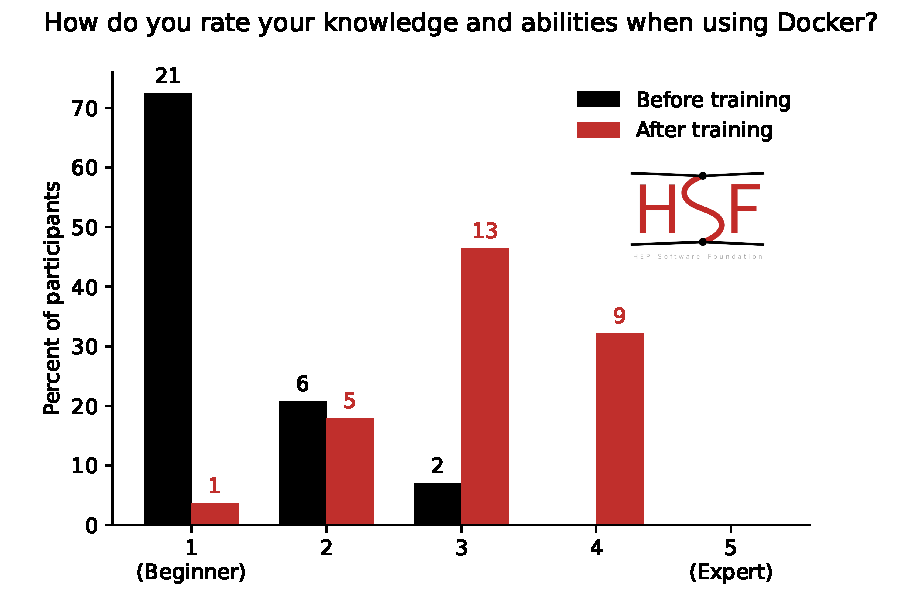
\includegraphics[width=11cm]{dockerfeedback_new.pdf}
\caption{The self-reported  pre- and post- training level of knowledge on the topic of Docker (a software container technology)
\label{fig:dockerfeedback}}
\end{figure*}
%
\section{Community}\label{sec:Community}
%
A workforce trained in a range of software skills with a combination of HEP domain knowledge and advanced software skills is the critical ingredient from which solutions to computing challenges can grow. To fulfill our mission, we rely on active community members~\cite{HSF-training-community} to support us in various ways, all of which, at this time are carried out on a voluntary basis but typically with dedication and enthusiasm; our community is intrinsically motivated. The members come from different HEP collaborations. This diversity adds great value to the training, as each brings their own flavor of experience from a different computing environment with a common goal to create, teach, and sustain a common set of skills across HEP. Recently, the Nuclear Physics community also became interested in our work and we hope that they will benefit from it given their similar software needs.  While training can impart and sharpen participants' software skills, it also gives tutors an opportunity to develop their pedagogical skills and professional profile. Given that the two-thirds of the HEP workforce eventually works outside of HEP, such as in the software industry and in data science, the HSF training will make a difference in robust preparation for such careers in terms of software knowledge and experience, and will enhance their chances of employability. The skills learnt, like Python, machine learning and data analysis, align with the needs of industry and strengthen the job profile of a physicist to work in industry.  The HSF community page carries links to the profile of each tutor that contributes to the training and serves as public proof of their capability and skills.


\section{Sustainability}\label{sec:Sustainability}

Sustainable software \cite{dan_katz}  gives HEP software developers an important skill that is essential to careers in the realm of software, inside or outside HEP. A sustainable training program~\cite{sustainability_flashtalk} is key to pursuing this goal. While continuing the existing work, it will be essential to  spread the training events and training expertise geographically to keep the costs low and move to an online training model to reduce financial burdens that accompany in-person training. In parallel, it is important that as the curriculum grows it begins to include material specifically aimed at making software sustainable.  Training should be structured so that a minimal set of people are needed to keep the training infrastructure running and identify additional costs for additional events. We need a long term funding model and one that migrates training from voluntary work rewarded by a picture on a webpage to tangible incentives, financial or otherwise. Mentoring the educators to grow the community is an important aspect of sustaining the workforce. In addition, giving them recognition can keep the community vibrant, motivated and help in careers. In this way, the community should recognize the broader value in our software training which prepares a workforce to solve computing challenges that are essential to advance our field and society at large.

To be able to lead software training across HEP and related communities over the long run, we must focus on building a community of individuals who are instructors, mentors, facilitators and participants (learners).  At the center must be a core team (supported directly by the HEP community for a long term) whose main focus is to support the overall mission of HEP software training. To achieve this, we need to build regional and local mentorship and leadership to train HEP communities that are guided and supported by the core team. Specifically, while we have started the following set of activities, we need to scale up by:

\begin{itemize} 
 
\item Engaging more HEP labs, institutes, and universities in this endeavour. 
\item Promote equity, diversity, inclusion and accessibility in participation across HEP communities and  be mindful of under-resourced institutions in different geographical regions.
\item Establish a mechanism to get feedback from our communities and improve the training.
\item Ensure that our core team and volunteers are afforded opportunities to grow professionally and have career paths.
\item Explore ways to manage a financial support model to share costs in the long term.

\end{itemize}

\section{Broader Impacts}\label{sec:BroaderImpacts}

HSF-led training is multilayered with a basic HEP software curriculum progressing to HEP specific physics tools. Integrated with this is a growing outreach program that is essential to building an influx of software workforce and training young minds, catching them early in their educational development. In addition, pursuing training in computing skills needed for researchers, several outreach events are organised on introducing python programming to K-12 teachers~\cite{HSF-training-DA-STEM-PR-2020} under IRIS-HEP and FIRST-HEP. The teachers can turn this into a classroom experience for their students where physics, astronomy and math courses can have problem solving components which integrate programming with python. In outreach events the teachers analyze physics data with Python programming using Google Colab and interpret their findings by making plots. Workshops teaching the basics of Machine Learning to school teachers are also organised~\cite{HSF-training-ML-STEM-PR-2021}. We plan to scale this experience by partnering with other stakeholders in HEP outreach, for example, Quarknet~\cite{quarknet}, which already has a well developed network of teachers and schools taking part in HEP outreach programs.

\section{Summary}\label{sec:Summary}

HSF and IRIS-HEP are creating software training and ensuring sustainability of software in HEP for years to come. The training material is open source and shared publicly via GitHub. This allows anyone to join the discussion and make contributions by proposing changes, thereby continuously improving the available material guided by continual feedback solicited from those engaged with the material and their implementation in training events. Finally, we have established a growing community of educators to broadly promote a culture within HEP that goes beyond valuing software skills, but also values the teaching of those skills to others. In doing so, we aim to foster a more active, inclusive, and diverse scientific community.  By leading software training across HEP and related communities, we will be able to meet the challenges in the field and beyond.

\section*{Acknowledgments}

This work is supported in part by National Science Foundation Cooperative Agreement OAC-1836650 and grants OAC-1829707 and OAC-1829729.



%Text with citations \cite{RefB} and \cite{RefJ}.
%\subsection{Subsection title}
%\label{sec:2}
%as required. Don't forget to give each section
%and subsection a unique label (see Sect.~\ref{sec:1}).
%\paragraph{Paragraph headings} Use paragraph headings as needed.
%\begin{equation}
%a^2+b^2=c^2
%\end{equation}

% For one-column wide figures use
%\begin{figure}
% Use the relevant command to insert your figure file.
% For example, with the graphicx package use
%  \includegraphics{example.eps}
% figure caption is below the figure
%\caption{Please write your figure caption here}
%\label{fig:1}       % Give a unique label
%\end{figure}
%
% For two-column wide figures use
%\begin{figure*}
% Use the relevant command to insert your figure file.
% For example, with the graphicx package use
% \includegraphics[width=0.75\textwidth]{example.eps}
% figure caption is below the figure
%\caption{Please write your figure caption here}
%\label{fig:2}       % Give a unique label
%\end{figure*}
%
% For tables use
%\begin{table}
% table caption is above the table
%\caption{Please write your table caption here}
%\label{tab:1}       % Give a unique label
% For LaTeX tables use
%\begin{tabular}{lll}
%\hline\noalign{\smallskip}
%first & second & third  \\
%\noalign{\smallskip}\hline\noalign{\smallskip}
%number & number & number \\
%number & number & number \\
%\noalign{\smallskip}\hline
%\end{tabular}
%\end{table}


%\begin{acknowledgements}
%If you'd like to thank anyone, place your comments here
%and remove the percent signs.
%\end{acknowledgements}


% Authors must disclose all relationships or interests that 
% could have direct or potential influence or impart bias on 
% the work: 
%
% \section*{Conflict of interest}
%
% The authors declare that they have no conflict of interest.


% BibTeX users please use one of
%\bibliographystyle{spbasic}      % basic style, author-year citations
%\bibliographystyle{spmpsci}      % mathematics and physical sciences
\bibliographystyle{spphys}       % APS-like style for physics
\bibliography{references}   % name your BibTeX data base

% Non-BibTeX users please use
%\begin{thebibliography}{}
%
% and use \bibitem to create references. Consult the Instructions
% for authors for reference list style.
%
%\bibitem{RefJ}
% Format for Journal Reference
%Author, Article title, Journal, Volume, page numbers (year)
% Format for books
%\bibitem{RefB}
%Author, Book title, page numbers. Publisher, place (year)
% etc
%\end{thebibliography}

\end{document}
% end of file template.tex

